\section{Continuous Actions with Actor-Critic}
DQN is great for discrete action spaces. However, it requires you to be able to calculate $\max_a Q(s, a)$ in closed form. Doing this is trivial for discrete action spaces (when you can just check which of the $n$ actions has the highest $Q$-value), but in continuous action spaces this is potentially a complex nonlinear optimization problem.

Actor-critic methods get around this by learning two networks: a $Q$-function, like DQN, and an explicit policy $\pi$ that is trained to maximize $\mathbb{E}_{a \sim \pi(a|s)} Q(s, a)$.

All parts in this section are run with the following command:
\begin{lstlisting}[language=bash,breaklines=true]
  python cs285/scripts/run_hw3_sac.py -cfg experiments/sac/<CONFIG>.yaml
\end{lstlisting}

\subsection{Implementation}
First, you'll need to take a look at the following files:
\begin{itemize}
    \item \verb|cs285/scripts/run_hw3_sac.py| - the main training loop for your SAC implementation.
    \item \verb|cs285/agents/soft_actor_critic.py| - the structure for the SAC learner you'll implement.
\end{itemize}
You may also find the following files useful:
\begin{itemize}
    \item \verb|cs285/networks/state_action_critic.py| - a simple MLP-based $Q(s, a)$ network. Note that unlike the DQN critic, which maps states to an array of $Q$-value, one per action, this critic maps one $(s, a)$ pair to a single $Q$-value.
    \item \verb|cs285/env_configs/sac_config.py| - base configuration (and list of hyperparameters).
    \item \verb|experiments/sac/*.yaml| - configuration files for the experiments.
\end{itemize}

You'll primarily be implementing your code in \verb|cs285/agents/soft_actor_critic.py|.

\textbf{Before implementing SAC:}
\begin{itemize}
    \item Fill in all of the \verb|TODO|s in \verb|cs285/scripts/run_hw3_sac.py|. This should look pretty similar to your DQN run script, as both are off-policy methods!
\end{itemize}

\subsubsection{Bootstrapping}
As in DQN, we train our critic by ``bootstrapping'' from a target critic. Using the tuple $(s_t, a_t, r_t, s_{t+1}, d_{t})$ (where $d_t$ is the flag for whether the trajectory terminates after this transition), we write:
\[y \gets r_t + \gamma (1-d_t) Q_\phi(s_{t+1}, a_{t+1}), a \sim \pi(a_{t+1}|s_{t+1})\]
\[\min_\phi (Q_\phi(s_t, a_t) - y)^2\]
In practice, we stabilize learning by using a separate \textit{target network} $Q_{\phi'}$. There are two common strategies for updating the target network:
\begin{itemize}
    \item \textit{Hard update} (like we implemented in DQN), where every $K$ steps we set $\phi' \gets \phi$.
    \item \textit{Soft update}, where $\phi'$ is continually updated towards $\phi$ with \textit{Polyak averaging} (exponential moving average). After each step, we perform the following operation:
    \[\phi' \gets \phi' + \tau(\phi-\phi')\]
\end{itemize}

\textbf{What you'll need to do} (in \verb|cs285/agents/soft_actor_critic.py|):
\begin{itemize}
    \item Implement the bootstrapped critic update in the \verb|update_critic| method.
    \item Update the critic for \verb|num_critic_updates| in the \verb|update| method.
    \item Implement soft and hard target network updates, depending on the configuration, in \verb|update|.
\end{itemize}

\textbf{Testing this section}:
\begin{itemize}
    \item Train an agent on \verb|Pendulum-v1| with the sample configuration \verb|experiments/sac/sanity_pendulum.yaml|. It shouldn't get high reward yet (you're not training an actor), but the $Q$-values should stabilize at some large negative number. The ``do-nothing'' reward for this environment is about -10 per step; you can use that together with the discount factor $\gamma$ to calculate (approximately) what $Q$ should be. If the $Q$-values go to minus infinity or stay close to zero, you probably have a bug.
\end{itemize}

\textbf{Deliverables}: None, once the critic is training as expected you can move on to the next section!

\subsubsection{Entropy Bonus and Soft Actor-Critic}
In DQN, we used an $\epsilon$-greedy strategy to decide which action to take at a given time. In continuous spaces, we have several options for generating exploration noise.

One of the most common is providing an \textit{entropy bonus} to encourage the actor to have high entropy (i.e. to be ``more random''), scaled by a ``temperature'' coefficient $\beta$. For example, in the REPARAMETRIZE case:
\[\mathcal L_\pi = Q(s, \mu_\theta(s) + \sigma_\theta(s)\epsilon) + \beta\mathcal{H}(\pi(a|s)).\]
Where entropy is defined as $\mathcal H(\pi(a|s)) = \mathbb{E}_{a \sim \pi}\left[-\log\pi(a|s)\right]$. To make sure entropy is also factored into the $Q$-function, we should also account for it in our target values:
\[y \gets r_t + \gamma(1-d_t)\left[Q_\phi(s_{t+1}, a_{t+1}) + \beta\mathcal{H}(\pi(a_{t+1}|s_{t+1}))\right]\]
When balanced against the ``maximize $Q$'' terms, this results in behavior where the actor will choose more random actions when it is unsure of what action to take.
Feel free to read more in the SAC paper: {\url{https://arxiv.org/abs/1801.01290 }}.

Note that maximizing entropy $\mathcal{H}(\pi_\theta) = -\mathbb{E}[\log \pi_\theta]$ requires differentiating \textit{through} the sampling distribution. We can do this via the ``reparametrization trick'' from lecture - if you'd like a refresher, skip to the section on REPARAMETRIZE.

\textbf{What you'll need to do} (in \verb|cs285/agents/soft_actor_critic.py|):
\begin{itemize}
    \item Implement \verb|entropy()| to calculate the approximate entropy of an actor distribution.
    \item Add the entropy term to the target critic values in \verb|update_critic()| and the actor loss in \verb|update_actor()|.
\end{itemize}

\textbf{Testing this section}:
\begin{itemize}
    \item The code should be logging \verb|entropy| during the critic updates. If you run \verb|sanity_pendulum.yaml| from before, it should achieve (close to) the maximum possible entropy for a 1-dimensional action space. Entropy is maximized by a uniform distribution:
    \[\mathcal{H}(\mathcal{U}[-1, 1]) = \mathbb{E}[-\log p(x)] = -\log \frac{1}{2} = \log 2 \approx 0.69\]
    Because currently our actor loss \textbf{only} consists of the entropy bonus (we haven't implemented anything to maximize rewards yet), the entropy should increase until it arrives at roughly this level.

    If your logged entropy is higher than this, or significantly lower, you have a bug.
\end{itemize}

\subsubsection{Actor with REINFORCE}
We can use the same REINFORCE gradient estimator that we used in our policy gradients algorithms to update our actor in actor-critic algorithms! We want to compute:
\[\nabla_\theta\mathbb{E}_{s \sim \mathcal{D}, a \sim \pi_\theta(a|s)}\left[Q(s, a)\right]\]
To do this using REINFORCE, we can use the policy gradient:
\[\mathbb{E}_{s \sim \mathcal{D}, a \sim \pi(a|s)}\left[\nabla_\theta \log(\pi_\theta(a|s))Q_\phi(s, a)\right]\]
Note that the actions $a$ are sampled from $\pi_\theta$, and we do \textbf{not} require real data samples. This means that to reduce variance we can just sample more actions from $\pi$ for any given state! You'll implement this in your code using the \verb|num_actor_samples| parameter.

\textbf{What you'll need to do} (in \verb|cs285/agents/soft_actor_critic.py|):
\begin{itemize}
    \item Implement the REINFORCE gradient estimator in the \verb|actor_loss_reinforce| method.
    \item Update the actor in \verb|update|.
\end{itemize}

\textbf{Testing this section}:
\begin{itemize}
    \item Train an agent on \verb|InvertedPendulum-v4| using \verb|sanity_invertedpendulum_reinforce.yaml|. You should achieve reward close to 1000, which corresponds to staying upright for all time steps.
\end{itemize}

\MYSOLUTION The result is shown below.

\begin{figure}[H]
    \centering
    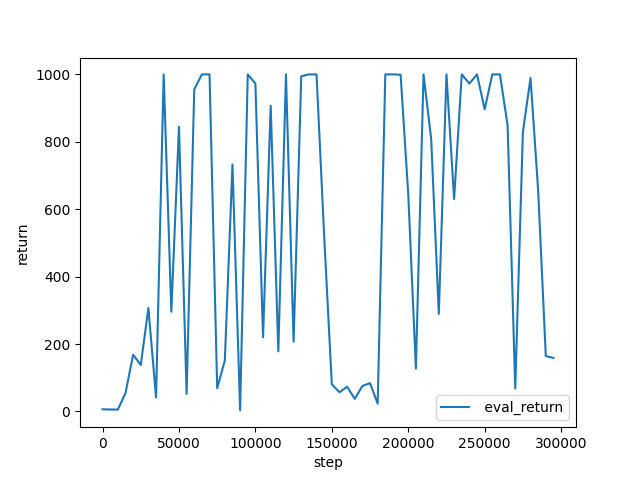
\includegraphics[width=0.6\textwidth]{../report/assets/P3-1-3-1.png}
    \caption{HalfCheetah-v4 with REINFORCE-1}
    \label{fig:halfcheetah-v4-reinforce-1}
\end{figure}

The problem is that the curve is very unstable! I can't tell the reason clearly. However, I did another experiment, which turns out to make the curve stable. The result is shown below.

\begin{figure}[H]
    \centering
    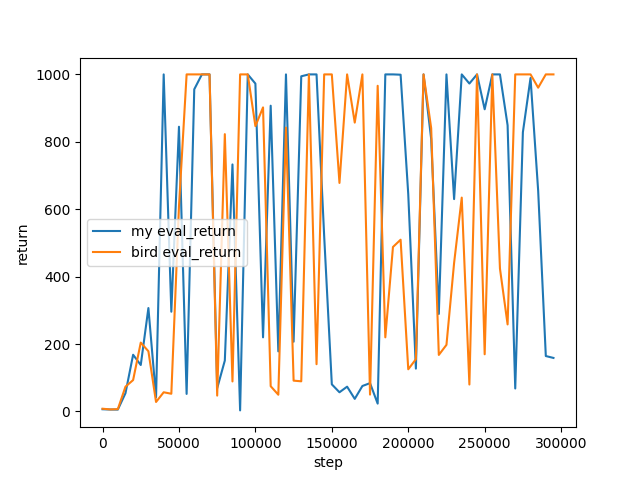
\includegraphics[width=0.45\textwidth]{../report/assets/P3-1-3-1-compare.png}
    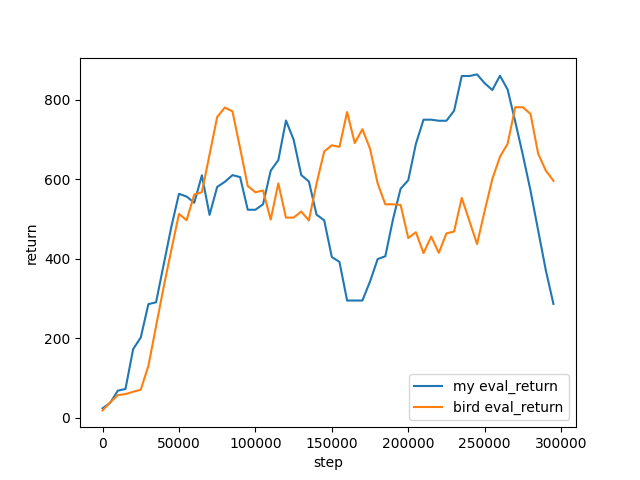
\includegraphics[width=0.45\textwidth]{../report/assets/P3-1-3-1-compare-smoothed.png}
    \caption{HalfCheetah-v4 with REINFORCE-1 (bird method); the right side is smoothed per 5 iterations}
    \label{fig:halfcheetah-v4-reinforce-1-another}
\end{figure}

The detail of the experiment is shown below: I changed the code as 
\begin{lstlisting}[language=Python]
def actor_loss_reinforce(self, obs: torch.Tensor):
    batch_size = obs.shape[0]

    action_distribution: torch.distributions.Distribution = self.actor(obs)

    with torch.no_grad():
        action = action_distribution.sample([self.num_actor_samples])
        assert action.shape == (
            self.num_actor_samples,
            batch_size,
            self.action_dim,
        ), action.shape
        if ptu.addition_args['bird method']:
            q_values = self.critic(torch.tile(obs,dims=(self.num_actor_samples,1,1)),action)
        else:
            q_values = self.target_critic(torch.tile(obs,dims= \
            
                    (self.num_actor_samples,1,1)),action)

        assert q_values.shape == (
            self.num_critic_networks,
            self.num_actor_samples,
            batch_size,
        ), q_values.shape

        q_values = torch.mean(q_values, axis=0)
        advantage = q_values

    log_probs = action_distribution.log_prob(action)
    loss = -torch.mean(log_probs*advantage)

    return loss, torch.mean(self.entropy(action_distribution))

\end{lstlisting}

In this function (also similarly in the function \verb|actor_loss_reparametrize|), If we use \verb|bird method|, then we use the \textbf{target critic} as the critic. Otherwise, we use the \textbf{critic} as the critic. 

In other words, my algorithm can be shown as

\begin{algorithm}[H]
    \caption{SAC Algorithm Implementation}
    \label{alg:sac}
    \begin{algorithmic}[1]
        \For{each step}
            \If {step $<$ some thereshold}
                \State Use random policy to collect data from the environment
            \Else
                \State Use the current policy to collect data from the environment
            \EndIf
            \State Insert the data into the replay buffer
            \If {step $<$ another thereshold}
                \State continue
            \EndIf
            \State Sample a batch of data from the replay buffer
            \State Update the critic for \textbf{num\_critic\_updates} times, using the actions from the actor
            \State Update the actor based on policy gradient or reparametrization trick with the objective being maximizing Q on \textcolor{red}{Target Critic Network}
            \State Perodically update (or momentum update) the target networks
        \EndFor
    \end{algorithmic}	
\end{algorithm}

The \verb|bird method| is almost the same, with only the red \textcolor{red}{Target Critic Network} changed to \textcolor{red}{Critic Network}. As XIBO (\url{github.com/szjzc2018}), an expert in RL, said,

\begin{quotation}
``Using the target network should be more stable.''
\end{quotation}

However, this contradicts the experiment results! So no one really know which method is really better.
    
\textbf{Deliverables}
\begin{itemize}
    \item Train an agent on \verb|HalfCheetah-v4| using the provided config (\verb|halfcheetah_reinforce1.yaml|). Note that this configuration uses only one sampled action per training example.
    \item Train another agent with \verb|halfcheetah_reinforce_10.yaml|. This configuration takes many samples from the actor for computing the REINFORCE gradient (we'll call this REINFORCE-10, and the single-sample version REINFORCE-1). Plot the results (evaluation return over time) on the same axes as the single-sample REINFORCE. Compare and explain your results.

\MYSOLUTION This figure (and the explanation) will be shown in section 3.1.4.
\end{itemize}

\subsubsection{Actor with REPARAMETRIZE}
REINFORCE works quite well with many samples, but particularly in high-dimensional action spaces, it starts to require a lot of samples to give low variance. We can improve this by using the reparametrized gradient. Parametrize $\pi_\theta$ as $\mu_\theta(s) + \sigma_\theta(s)\epsilon$, where $\epsilon$ is normally distributed. Then we can write:
\[\nabla_\theta\mathbb{E}_{s \sim \mathcal{D}, a \sim \pi_\theta(a|s)}\left[Q(s, a)\right] = \nabla_\theta\mathbb{E}_{s \sim \mathcal{D}, \epsilon \sim \mathcal{N}}\left[Q(s, \mu_\theta(s) + \sigma_\theta(s)\epsilon))\right] = \mathbb{E}_{s \sim \mathcal{D}, \epsilon \sim \mathcal{N}}\left[\nabla_\theta Q(s, \mu_\theta(s) + \sigma_\theta(s)\epsilon))\right]\]
This gradient estimator often gives a much lower variance, so it can be used with few samples (in practice, just using a single sample tends to work very well).

\textbf{Hint}: you can use \verb|.rsample()| to get a \textit{reparametrized} sample from a distribution in PyTorch.

\textbf{What you'll need to do}:
\begin{itemize}
    \item Implement \verb|actor_loss_reparametrize()|. Be careful to use the reparametrization trick for sampling!
\end{itemize}

\textbf{Testing this section}:
\begin{itemize}
    \item Make sure you can solve \verb|InvertedPendulum-v4| (use \verb|sanity_invertedpendulum_reparametrize.yaml|) and achieve similar reward to the REINFORCE case.
\end{itemize}

\MYSOLUTION The plot is shown below.

\begin{figure}[H]
    \centering
    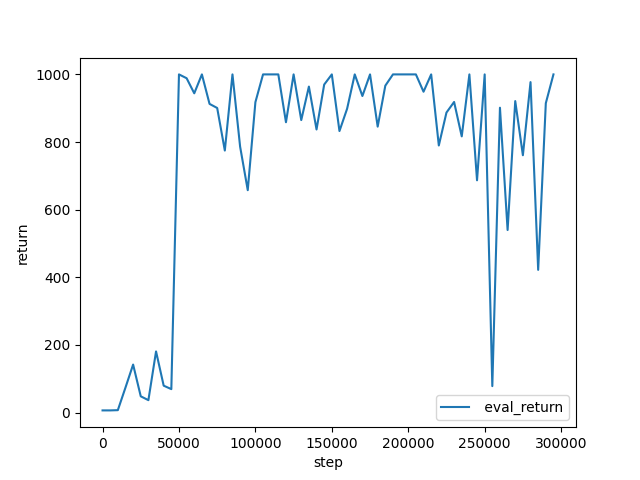
\includegraphics[width=0.6\textwidth]{../report/assets/P3-1-4-1.png}
    \caption{InvertedPendulum-v4 with REPARAMETRIZE}
    \label{fig:invert-v4-reparametrize}
\end{figure}

\textbf{Deliverables}: 
\begin{itemize}
    \item Train (once again) on \verb|HalfCheetah-v4| with \verb|halfcheetah_reparametrize.yaml|. Plot results for all three gradient estimators (REINFORCE-1, REINFORCE-10 samples, and REPARAMETRIZE) on the same set of axes, with number of environment steps on the $x$-axis and evaluation return on the $y$-axis.

\MYSOLUTION The plot is shown below.

\begin{figure}[H]
    \centering
    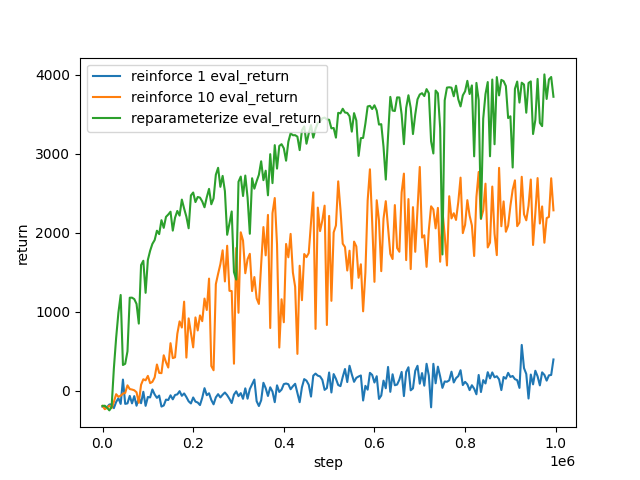
\includegraphics[width=0.6\textwidth]{../report/assets/P3-1-4-2.png}
    \caption{HalfCheetah-v4 with REPARAMETRIZE and two REINFORCE methods}
    \label{fig:halfcheetah-v4-reparametrize}
\end{figure}

For explanation (of the 3.1.3 section), the REINFORCE-10 method is better than REINFORCE-1 method, since there are more samples for REINFORCE-10 method.

    \item Train an agent for the \verb|Humanoid-v4| environment with \verb|humanoid_sac.yaml| and plot results.
    
\MYSOLUTION

This graph will be put in 3.1.5 section.

\end{itemize}

\subsubsection{Stabilizing Target Values}
As in DQN, the target $Q$ with a single critic exhibits \textit{overestimation bias}! There are a few commonly-used strategies to combat this:
\begin{itemize}
    \item Double-$Q$: learn two critics $Q_{\phi_A}, Q_{\phi_B}$, and keep two target networks $Q_{\phi_A'}, Q_{\phi_B'}$. Then, use $Q_{\phi'_A}$ to compute target values for $Q_{\phi_B}$ and vice versa:
    \[y_A = r + \gamma Q_{\phi_B'}(s', a')\]
    \[y_B = r + \gamma Q_{\phi_A'}(s', a')\]
    \item \textit{Clipped} double-$Q$: learn two critics $Q_{\phi_A}, Q_{\phi_B}$ (and keep two target networks). Then, compute the target values as $\min(Q_{\phi_A'}, Q_{\phi_B'})$.
    \[y_A = y_B = r + \gamma \min\left(Q_{\phi_A'}(s', a'), Q_{\phi_B'}(s', a')\right)\]
    \item \textbf{(Optional, bonus)} \textit{Ensembled} clipped double-$Q$: learn many critics (10 is common) and keep a target network for each. To compute target values, first run all the critics and sample two $Q$-values for each sample. Then, take the minimum (as in clipped double-$Q$). If you want to learn more about this, you can check out ``Randomized Ensembled Double-Q'': \url{https://arxiv.org/abs/2101.05982}.
\end{itemize}
Implement double-$Q$ and clipped double-$Q$ in the \verb|q_backup_strategy| function in \verb|soft_actor_critic.py|.

\textbf{Deliverables}:
\begin{itemize}
    \item Run single-$Q$, double-$Q$, and clipped double-$Q$ on \verb|Hopper-v4| using the corresponding configuration files. Which one works best? Plot the logged \verb|eval_return| from each of them as well as \verb|q_values|. Discuss how these results relate to overestimation bias.
    
\MYSOLUTION Among the four implementations, double-Q and REDQ works the best. The plot is shown below.

\begin{figure}[H]
    \centering
    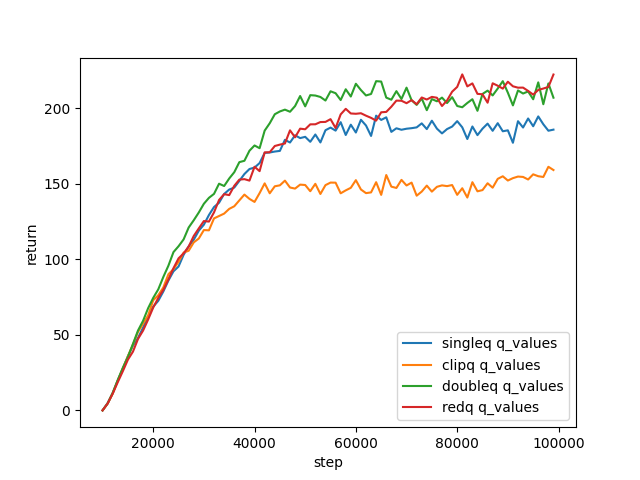
\includegraphics[width=0.4\textwidth]{../report/assets/P3-1-5-1.png}
    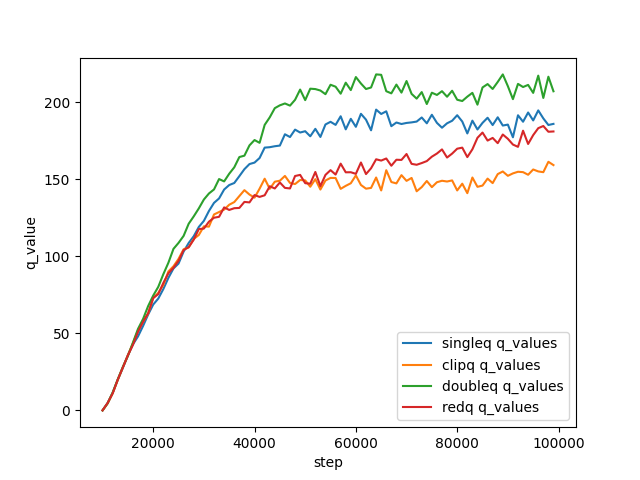
\includegraphics[width=0.4\textwidth]{../report/assets/P3-1-5-2.png}
    \caption{Hopper-v4 with single-Q, double-Q, clipped double-Q and REDQ}
    \label{fig:hopper-v4-q}
\end{figure}

From the plot of the Q values, at first glance, it seems that the double Q has largest Q values. This seems to contradict the fact that double Q reduces the Q function. However, this may due to the fact that double Q method performs best, so the Q values increase very quickly. Thus, from the Q values, we can't really tell much. On the other hand, from the performance figure, we can see that double Q indeed performs the best.

    \item Pick the best configuration (single-$Q$/double-$Q$/clipped double-$Q$, or REDQ if you implement it) and run it on \verb|Humanoid-v4| using \verb|humanoid.yaml| (edit the config to use the best option). You can truncate it after 500K environment steps. If you got results from the humanoid environment in the last homework, plot them together with environment steps on the $x$-axis and evaluation return on the $y$-axis. Otherwise, we will provide a humanoid log file that you can use for comparison. How do the off-policy and on-policy algorithms compare in terms of sample efficiency? \textit{Note: if you'd like to run training to completion (5M steps), you should get a proper, walking humanoid! You can run with videos enabled by using \texttt{-nvid 1}. If you run with videos, you can strip videos from the logs for submission with \href{https://gist.github.com/kylestach/e9964f5f34ee74367547dec83eaf5fae}{this script}.}
    
\MYSOLUTION 

\begin{figure}[H]
    \centering
    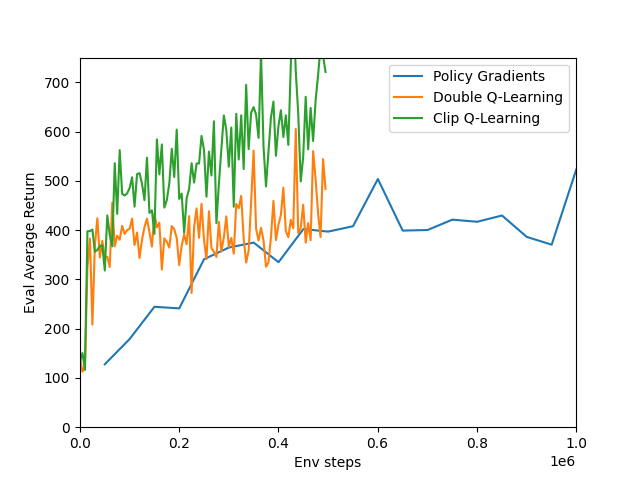
\includegraphics[width=0.6\textwidth]{../report/assets/3-1-5-3.png}
    \caption{Humanoid-v4 with double-Q}
    \label{fig:humanoid-v4-q}
\end{figure}

It is clear that off-policy methods are more sample efficient than on-policy methods. However, since the computation power is limited, I can't run the off-policy method to the end, so I can't tell which method is better in the end.
\end{itemize}